\documentclass{beamer}

\usepackage{tikz}
\usetikzlibrary{shapes}

\usepackage{framed,color,verbatim}
\definecolor{shadecolor}{rgb}{.9, .9, .9}
\newenvironment{code}%
   {\snugshade\verbatim}%
   {\endverbatim\endsnugshade}

\usetheme{Boadilla}
\usecolortheme{crane}
% \setbeameroption{show notes on second screen}

\title{SSH Monitor}
\subtitle{Web development final project}
\author{atmatto}
\date{}

\begin{document}

\frame{\titlepage}

\begin{frame}[fragile]
	\frametitle{SSH Setup}
	Install the SSH server
	\begin{code}sudo apt install openssh-server\end{code}
	Restart the system
	\begin{code}shutdown -r now\end{code}
	Check if the server is properly installed and activated
	\begin{code}
		systemctl is-active ssh
		ssh localhost
	\end{code}
\end{frame}

\begin{frame}[fragile]
	\frametitle{Connecting to the VM}
	Check the IP address of the VM
	\begin{code}
	$ nmcli
	enp1s0: connected to Wired connection 1
	        ...
	        inet4 192.168.122.39/24
	        ...
	\end{code}
	Connect to the VM from another system
	\begin{code}ssh user@vm.ip.address\end{code}
\end{frame}

\begin{frame}[fragile]
	\frametitle{SSH Configuration}
	\framesubtitle{Setting the port number}
	Edit the configuration
	\begin{code}
		sudo nano /lib/systemd/system/ssh.socket
		...
		[Socket]
		ListenStream=2244
		...
	\end{code}
	Reload the configuration
	\begin{code}
		sudo systemctl daemon-reload
		sudo systemctl restart ssh.socket
	\end{code}
	Connect
	\begin{code}ssh user@vm.ip.address -p 2244\end{code}
	% Firewall (set, check)
\end{frame}

\begin{frame}[fragile]
	\frametitle{SSH Configuration}
	\framesubtitle{Setting the banner}
	To set a message to be displayed before the login prompt:
	\begin{code}
		sudo nano /etc/ssh/sshd_config
	\end{code}
	Uncomment and set the path
	\begin{code}
		...
		Banner /etc/ssh-banner
		...
	\end{code}
	Set the message
	\begin{code}
		sudo nano /etc/ssh-banner
	\end{code}
	\includegraphics[width=0.4\textwidth]{banner.png}
\end{frame}

\begin{frame}[fragile]
	\frametitle{PuTTY}
	\begin{columns}
		\begin{column}{0.7\textwidth}
			Check the IP address of the VM
			\begin{code}
			$ nmcli
			enp1s0: connected to Wired connection 1
			        ...
			        inet4 192.168.122.39/24
			        ...
			\end{code}
			Connect from Windows to the VM using PuTTY\\
		\end{column}
		\begin{column}{0.3\textwidth}
			\includegraphics[width=\textwidth]{putty.png}
		\end{column}
	\end{columns}
	\vspace{0.5cm}
	\begin{center}
		\includegraphics[width=0.5\textwidth]{putty-zoom.png}
	\end{center}
\end{frame}

\begin{frame}[fragile]
	\frametitle{Web app}
	\framesubtitle{Features}
	\begin{center}
		\includegraphics[width=0.5\textwidth]{sshmon.png}
	\end{center}
	\begin{itemize}
		\item A web app served on the network
		\item Displaying output of Linux commands in a graphical way, letting the user analyse the configuration
		\begin{center}
			service status and log, configuration, port number, connected users, network devices and IP addresses, key fingerprints
		\end{center}
		\item Downloading manuals from the server
	\end{itemize}
\end{frame}

\begin{frame}[fragile]
	\frametitle{Web app}
	\framesubtitle{Front end}
	\begin{center}
		\includegraphics[width=0.8\textwidth]{app.png}
	\end{center}
\end{frame}

\begin{frame}[fragile]
	\frametitle{Web app}
	\framesubtitle{Front end}
	\begin{columns}
		\begin{column}{0.6\textwidth}
			\begin{itemize}
				\item<1-> Multiple pages with a navigation bar
				\item<2-> Code blocks
				\item<3-> Text decorations
				\item<4-> Borders
				\item<5-> Tables
				\item<6-> Lists
				\item<7-> Animations
			\end{itemize}
		\end{column}
		\begin{column}{0.4\textwidth}
			\includegraphics<1>[width=\textwidth]{navigation.png}
			\hspace{-3cm}
			\includegraphics<2>[width=1.55\textwidth]{code.png}
			\hspace{3cm}
			\includegraphics<3>[width=\textwidth]{text.png}
			\includegraphics<4>[width=\textwidth]{borders.png}
			\includegraphics<5>[width=\textwidth]{table.png}
			\includegraphics<6>[width=\textwidth]{list.png}
		\end{column}
	\end{columns}
\end{frame}

\begin{frame}[fragile]
	\frametitle{Web app}
	\framesubtitle{Back end}
	Web application written in Go
	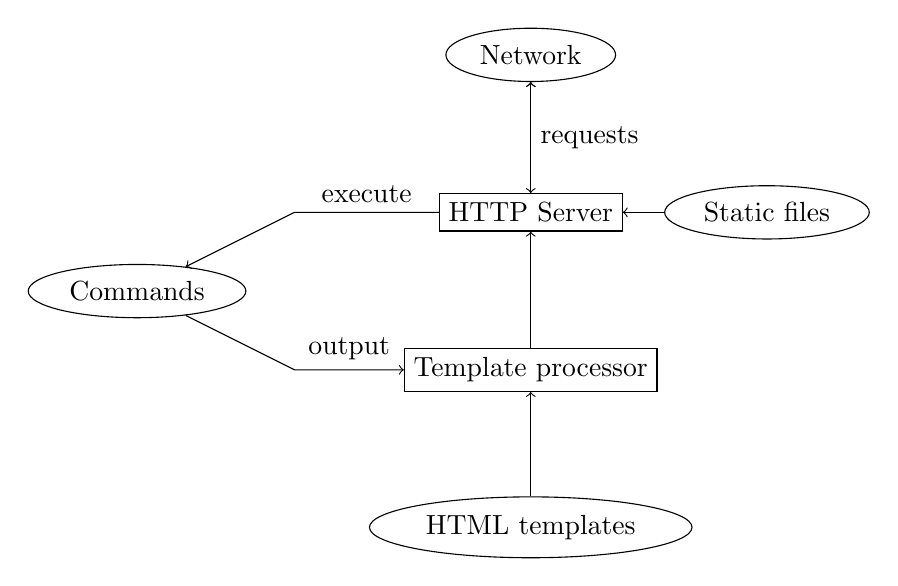
\begin{tikzpicture}
		\path (0, 0) node(net) [ellipse, draw] {Network};
		\path (0, -2) node(srv) [rectangle, draw] {HTTP Server};
		\path (0, -4) node(tp) [rectangle, draw] {Template processor};
		\path (0, -6) node(html) [ellipse, draw] {HTML templates};
		\path (-5, -3) node(cmd) [ellipse, draw] {Commands};
		\path (3, -2) node(st) [ellipse, draw] {Static files};
		\draw [<->] (srv) to node[right] {requests} (net);
		\draw [->] (srv) to (net);
		\draw [->] (srv) to node[above] {execute} (-3, -2) to (cmd);
		\draw [->] (tp) to (srv);
		\draw [->] (st) to (srv);
		\draw [->] (html) to (tp);
		\draw [->] (cmd) to (-3, -4) to node[above] {output} (tp);
	\end{tikzpicture}
\end{frame}

\begin{frame}[fragile]
	\begin{center}
	Thank you for your attention
	\end{center}
\end{frame}

\end{document}
